\documentclass[conference]{IEEEtran}

\IEEEoverridecommandlockouts

\usepackage{cite}
\usepackage{amsmath,amssymb,amsfonts}
\usepackage{algorithmic}
\usepackage{graphicx}
\usepackage{textcomp}
\usepackage{xcolor}

\usepackage{booktabs} %@{}
\usepackage{pgfplots}
\pgfplotsset{compat=1.16}
\usepackage[per-mode=symbol,detect-all]{siunitx}
\usepackage{hyperref}
\usepackage{cleveref} %\Cref{} vs. \cref{}
\usepackage[protrusion=true,expansion=true]{microtype}
\usepackage{mathabx} % for \bigtimes


\def\BibTeX{{\rm B\kern-.05em{\sc i\kern-.025em b}\kern-.08em
    T\kern-.1667em\lower.7ex\hbox{E}\kern-.125emX}}

\begin{document}


\title{\LARGE \textbf{Active Learning of Global Metamodels} 
%\thanks{Ross Alexander is supported by a Stanford Graduate Fellowship (SGF) in Science and Engineering.}
}


\author{\IEEEauthorblockN{  Ross Alexander}
\IEEEauthorblockA{\textit{  Department of Aeronautics and Astronautics} \\
\textit{                    Stanford University} \\
                            Stanford, CA 94305 \\
                            rbalexan@stanford.edu}} % or ORCID


\maketitle

\section{Project Update}
\label{sec:update}

% What you have been able to accomplish
\subsection{Progress So Far}
Previously, we proposed to explore neural networks (NNs), Gaussian processes (GPs), and their deep variants (DNNs and DGPs) in global metamodeling tasks with active learning. Global metamodeling is the discipline concerned with constructing a surrogate model over the input space that is optimal with respect to the number of training examples. We employ active learning in global metamodeling (also called adaptive sampling) to improve sample efficiency and thus, optimality of the metamodel.

So far, we have implemented variance-based adaptive sampling for GPs on several 1D and 2D functions. First, we generate a small initial set of design points and objective function evaluations (e.g. a dataset $\mathcal{D} = \{(x^{(i)}, y^{(i)})\}$) using a random sampling approach. We provide the initial sample set and fit a GP to the samples. We then evaluate the GP over a uniform grid to determine the next sample location according the variance-based exploration strategy. Following this, we continually add the requested sample, re-fit the GP, and identify a new sample.

Figure \ref{fig:sinc-gp} shows five iterations of active learning on the 1D $\text{sinc}(x)$ function that was initialized with 12 random samples over the domain. We can see that the variance-based method performs well and quickly learns a good metamodel. Similarly, we show a single iteration of active learning on 2D Franke function in Figure \ref{fig:franke-gp}. We are observing the cubic evaluation complexity, so extensions to higher dimensions is currently limited.

Some new additional directions to explore include generating the initial dataset using a central composite design, which could improve performance by reducing adaptive samples requested on the design space boundaries. Additionally, we may formulate a method to select samples based on expected improvement in integrated variance.

% a revised timeline to completion
\subsection{Work Ahead}
We should be able to at least complete a comparison between GPs and NNs, between GPs and DGPs, or between GPs with various adaptive sampling approaches. This will require developing the NN or DGP code along with coding up the calculation of performance metrics (i.e. RMSE, ISE, IV, and model generation time). We should have some results for these metamodels and active learning techniques on several general optimization benchmark functions of varying dimensionality and modality.

\vspace*{-2em}
\begin{figure}[htbp]
    \centering
    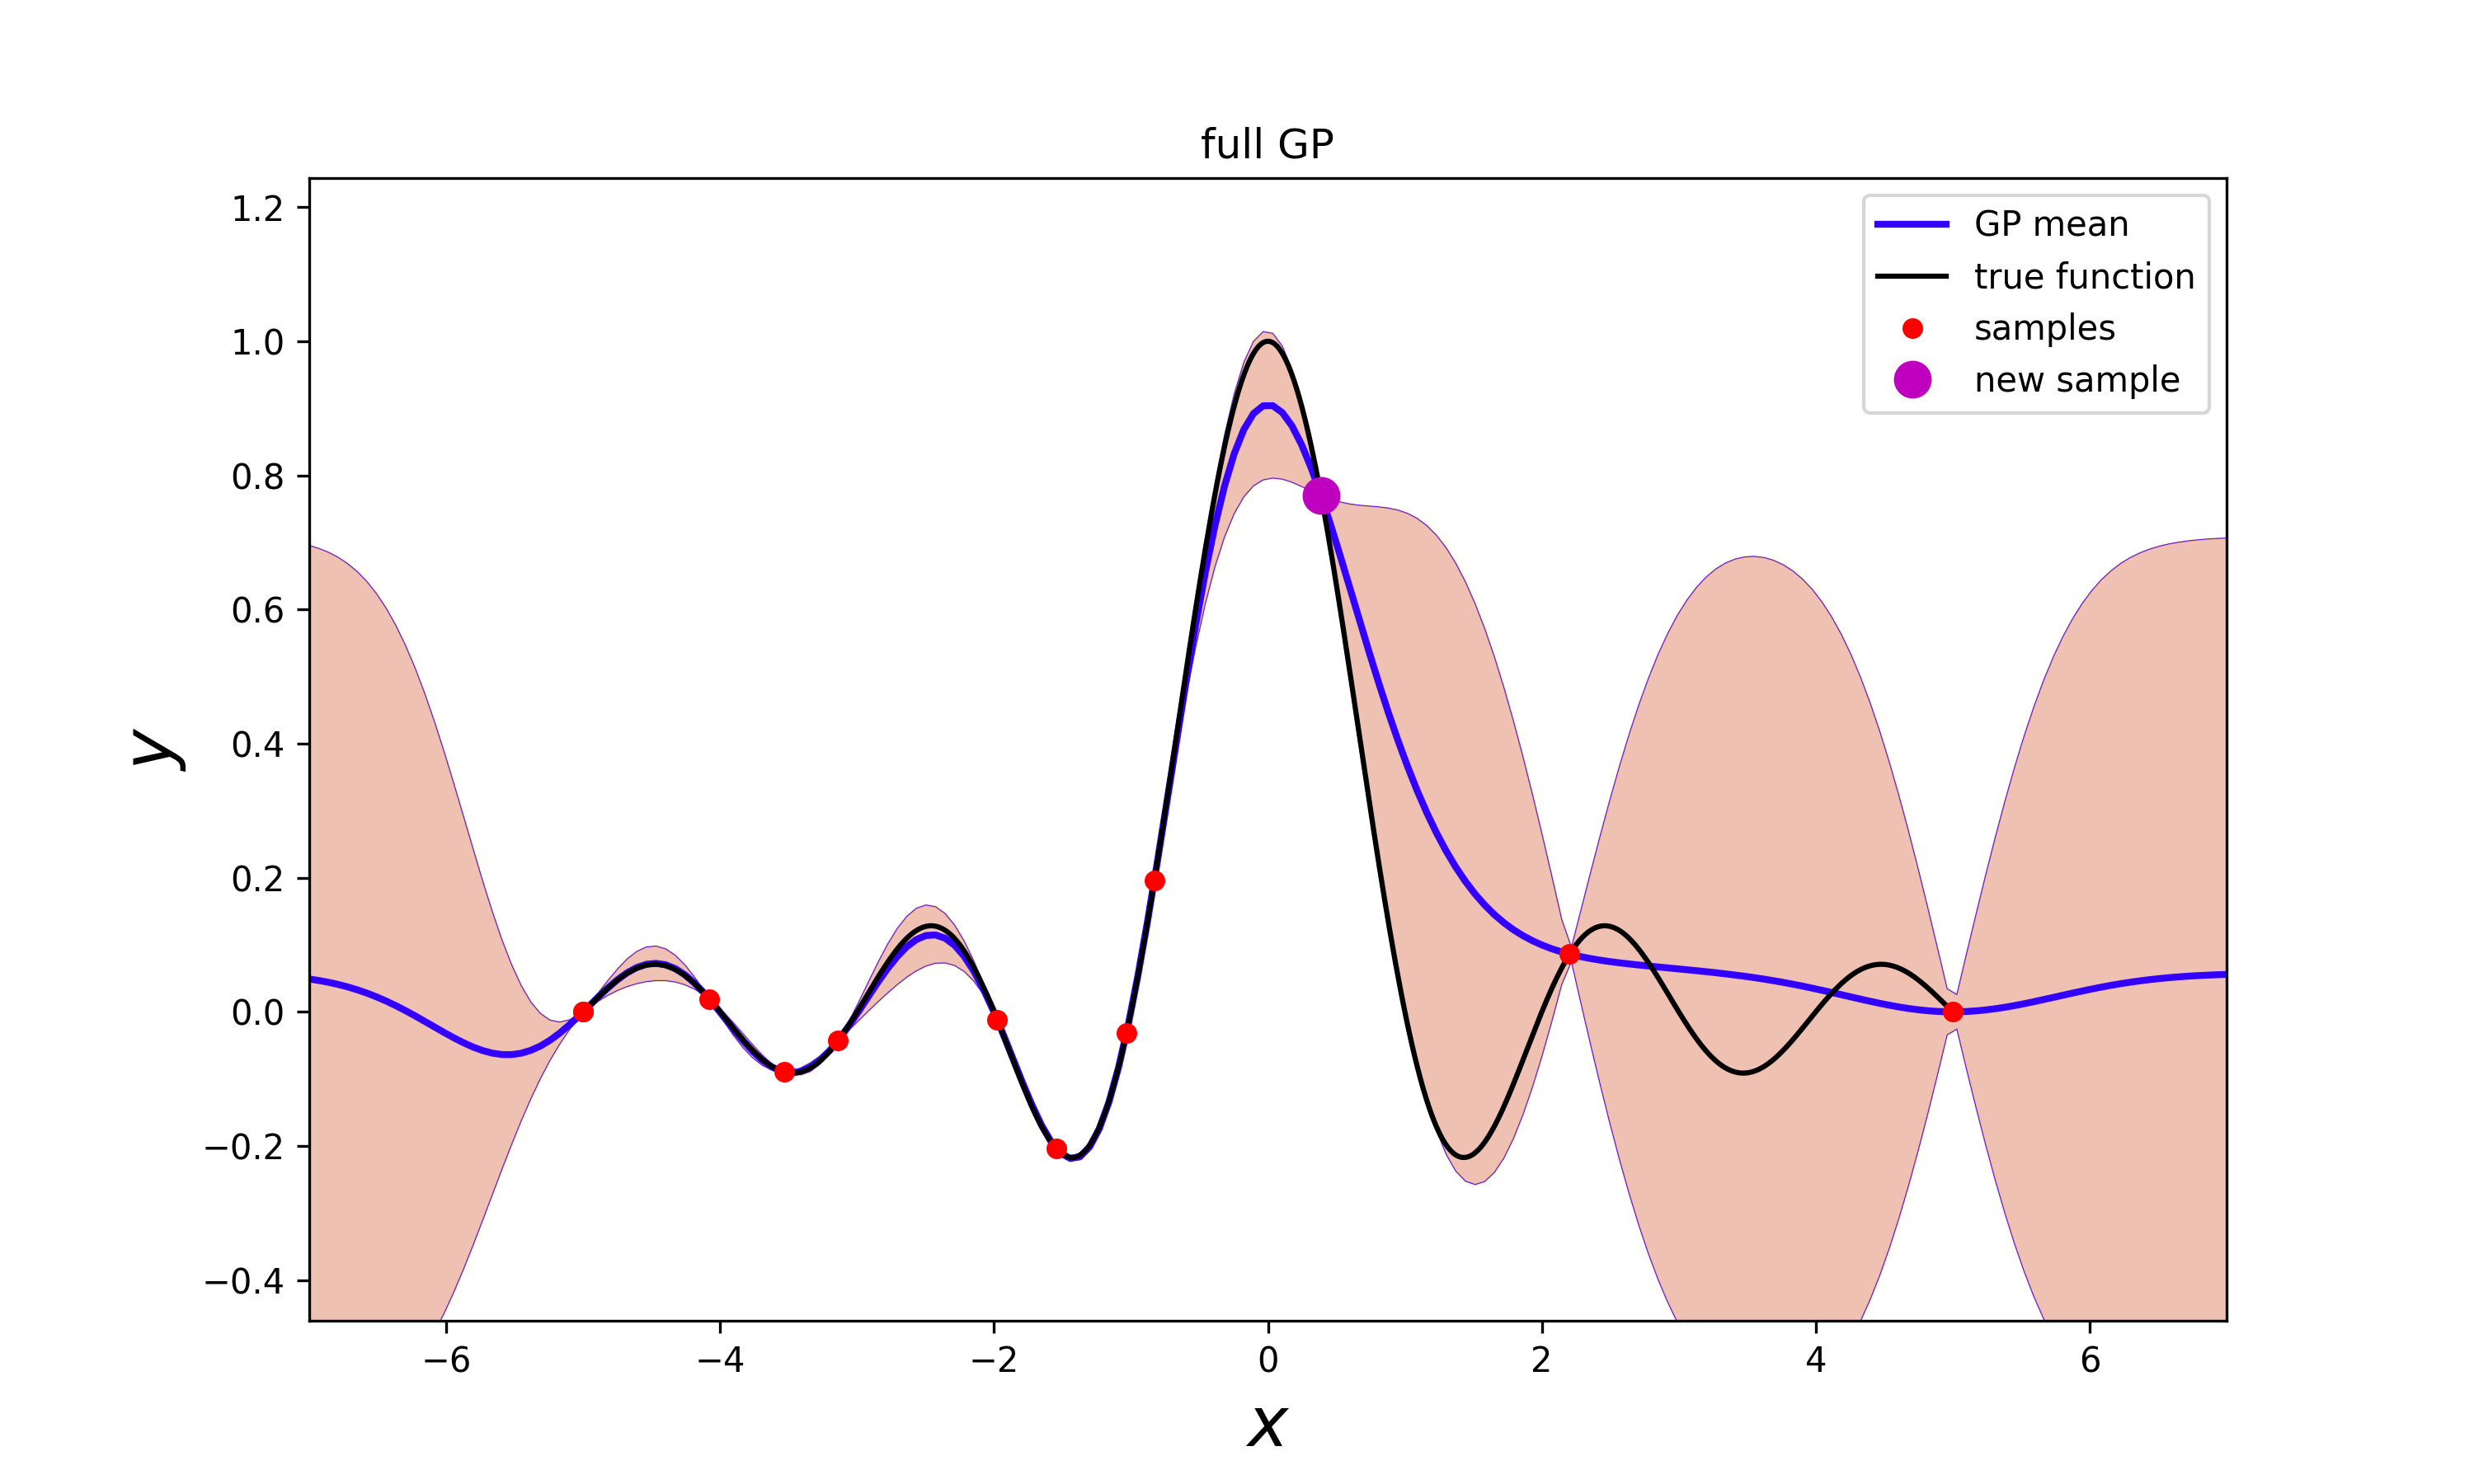
\includegraphics[width=0.74\linewidth]{final-project/update/plots/gp-12to20-pt12.png} \vspace*{-1em} \\
    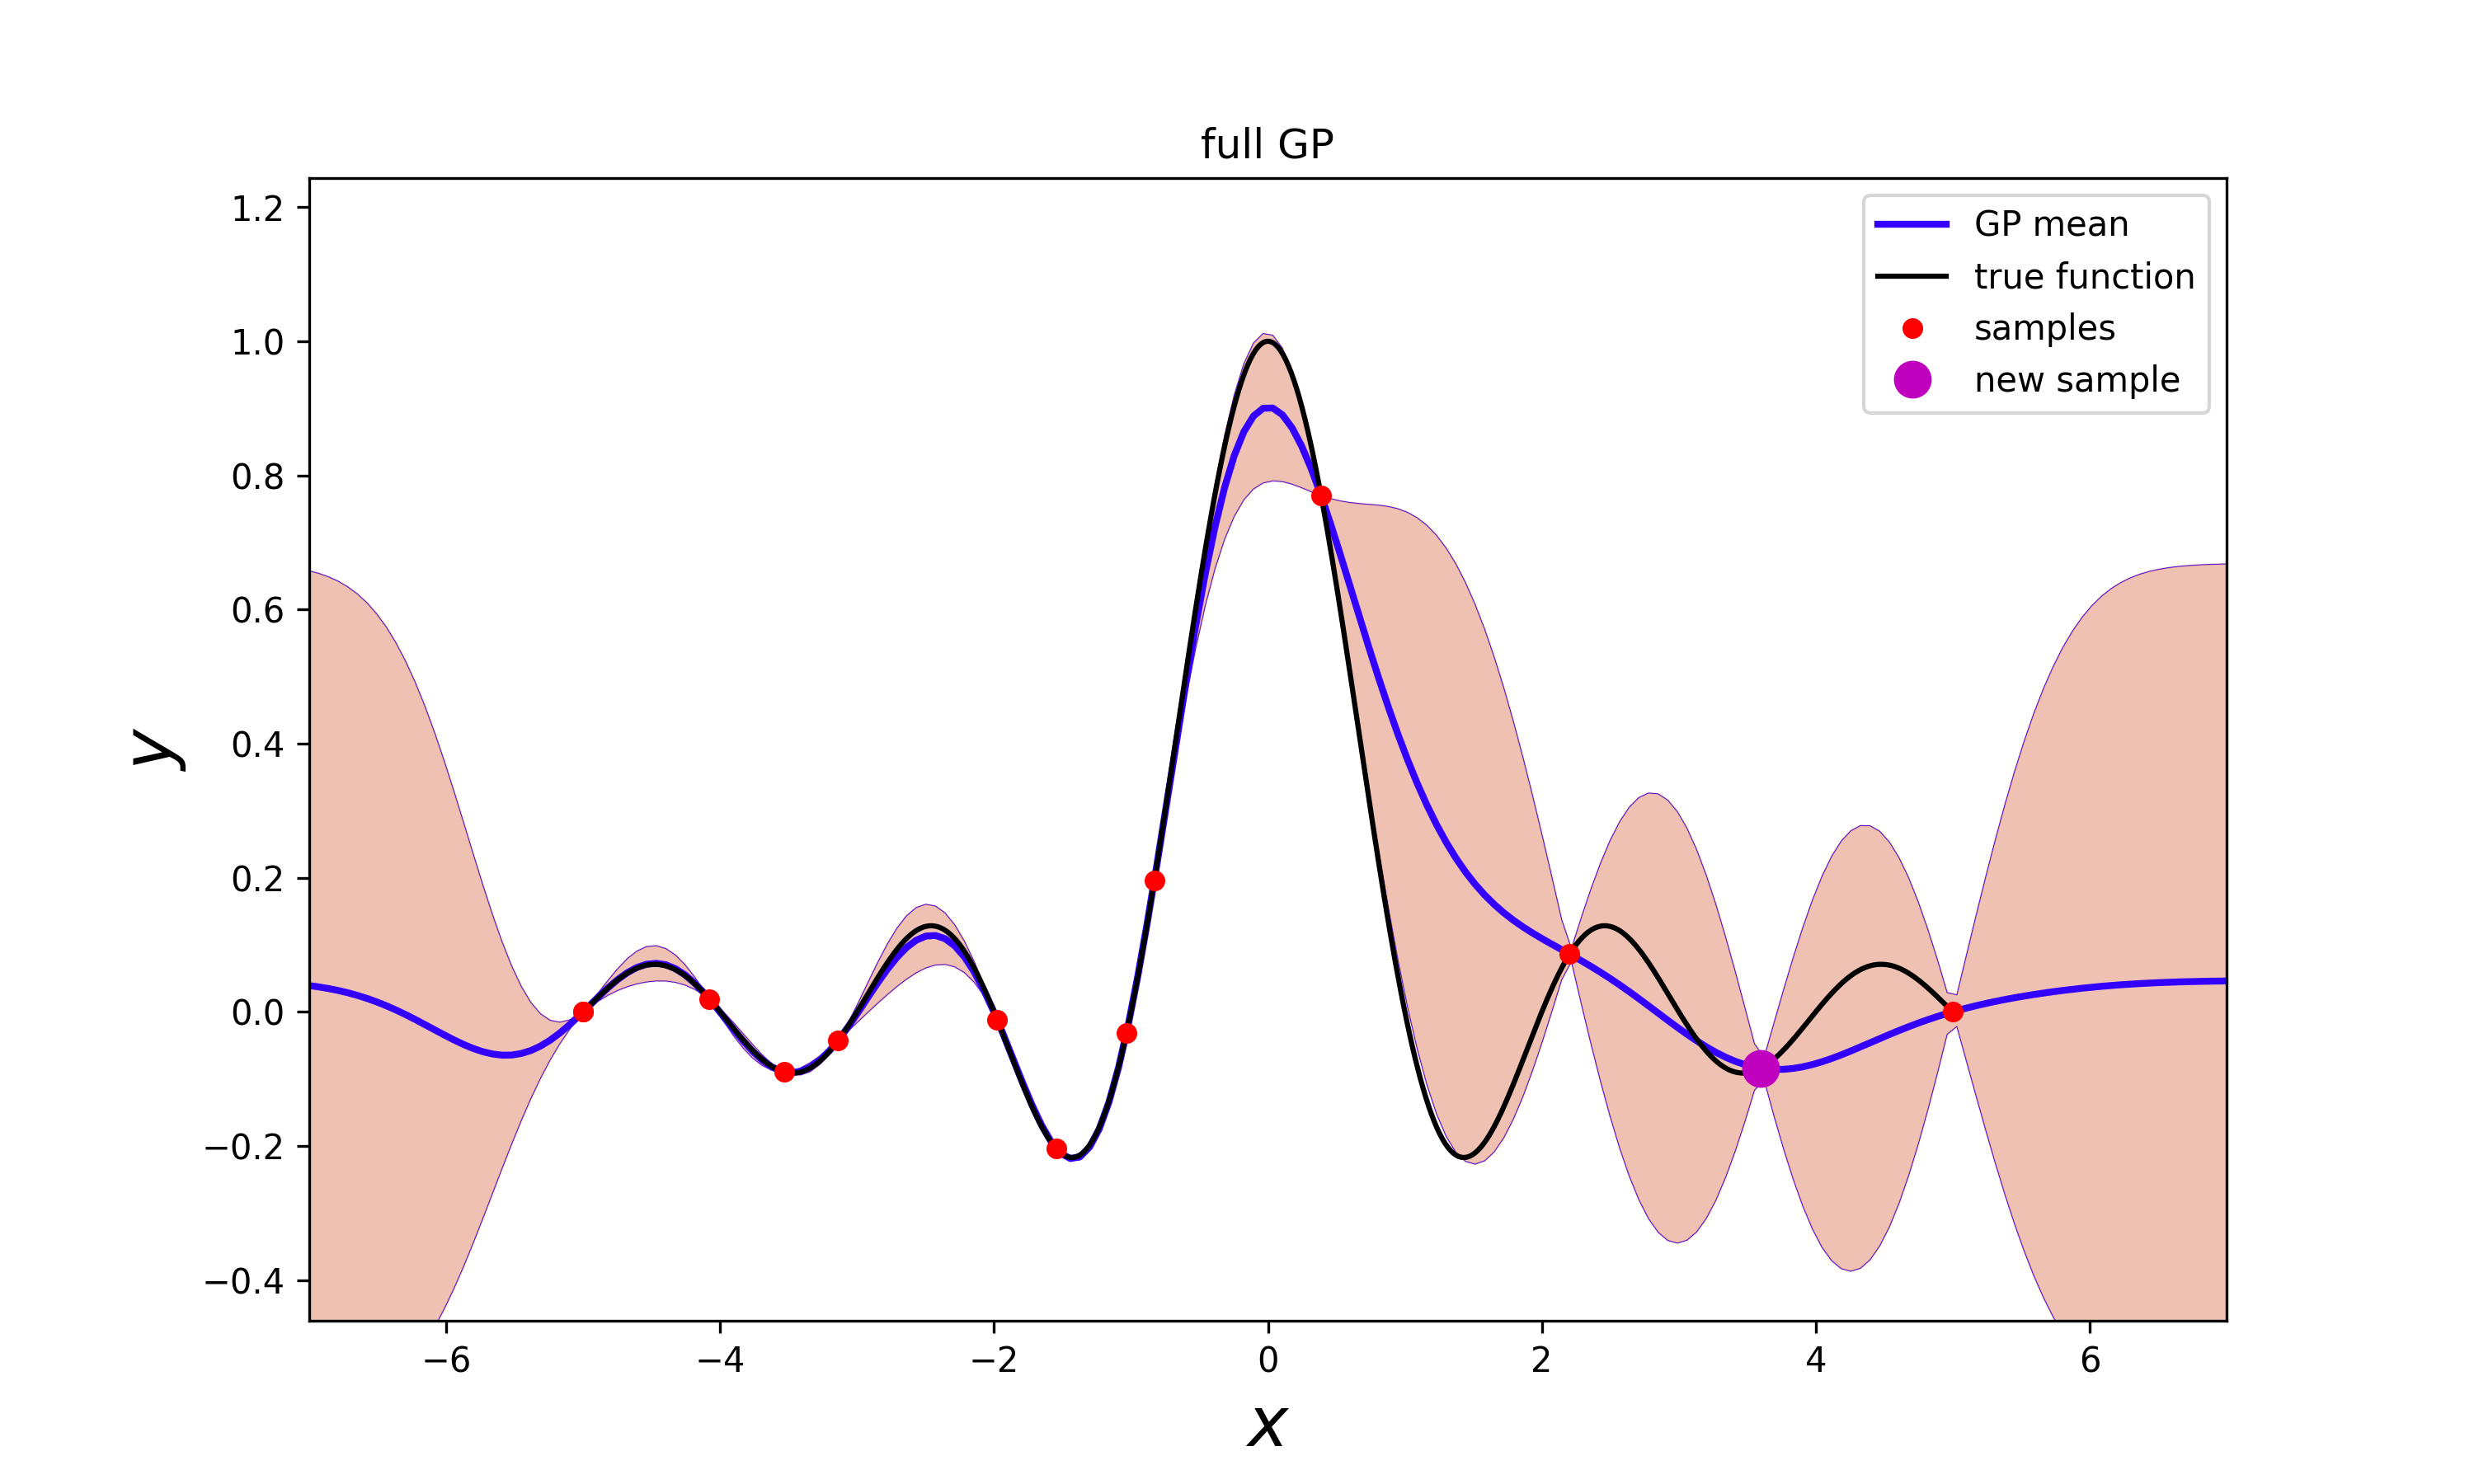
\includegraphics[width=0.74\linewidth]{final-project/update/plots/gp-12to20-pt13.png} \vspace*{-1em} \\
    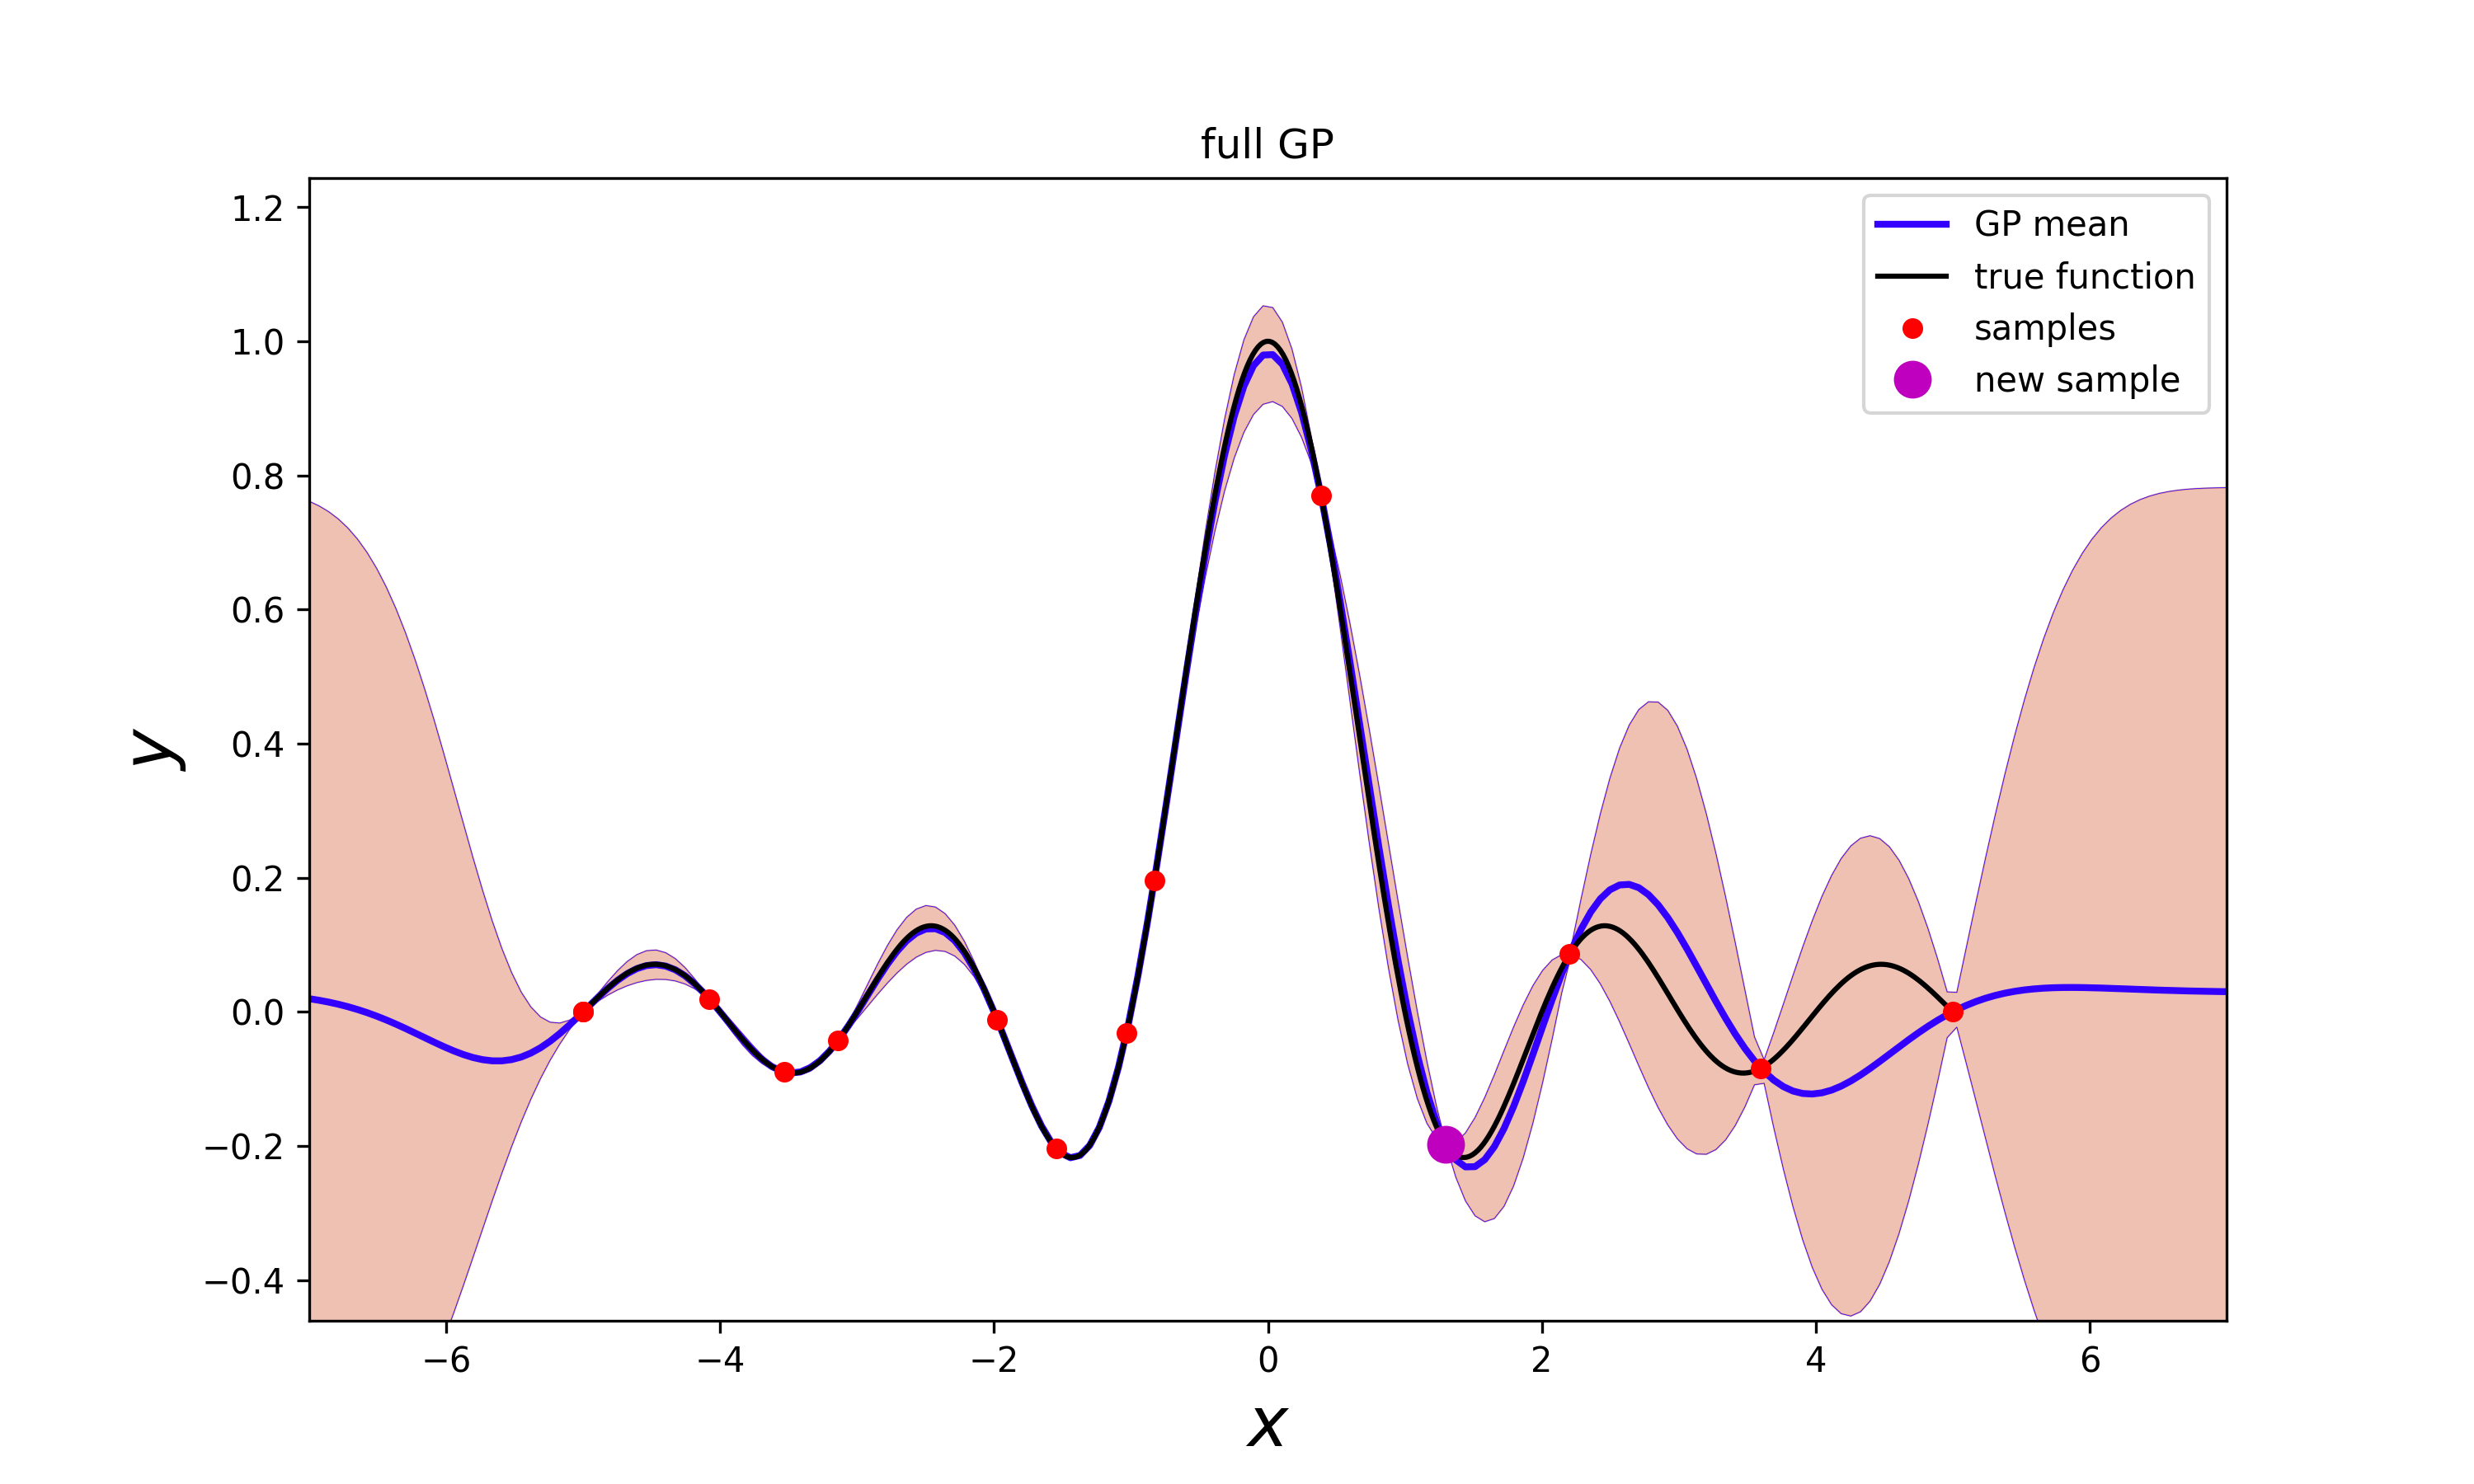
\includegraphics[width=0.74\linewidth]{final-project/update/plots/gp-12to20-pt14.png} \vspace*{-1em} \\
    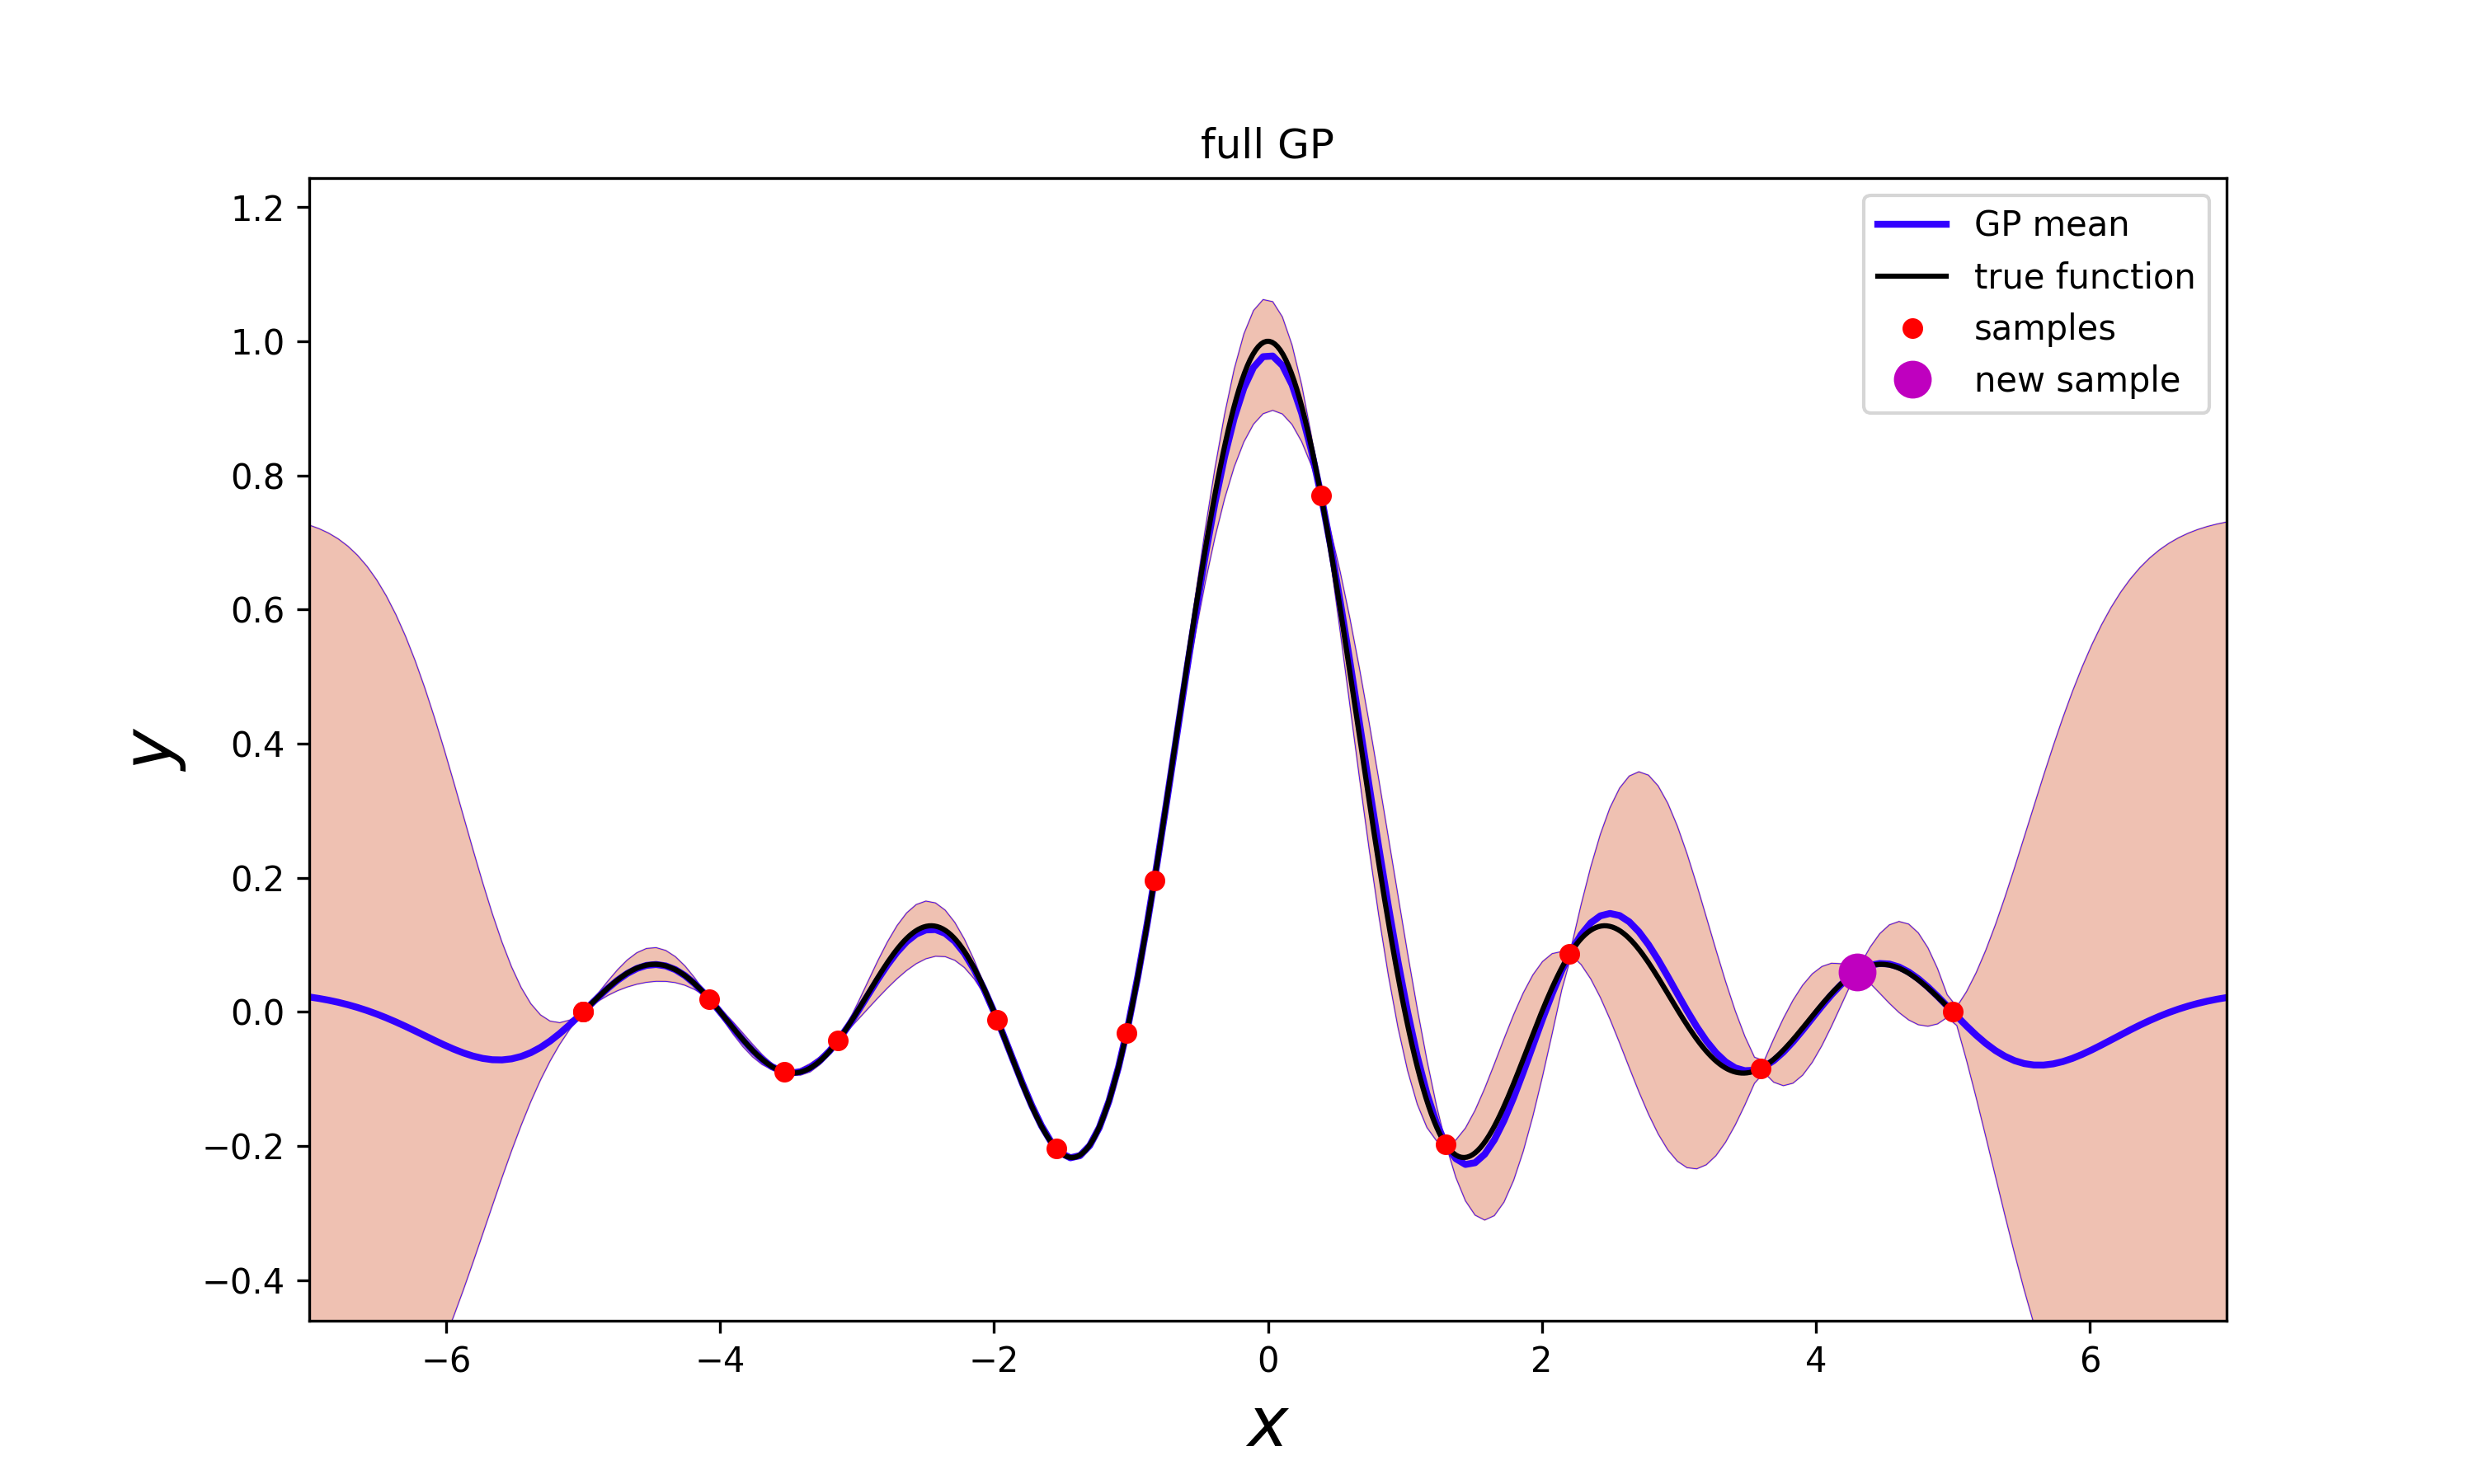
\includegraphics[width=0.74\linewidth]{final-project/update/plots/gp-12to20-pt15.png} \vspace*{-1em} \\
    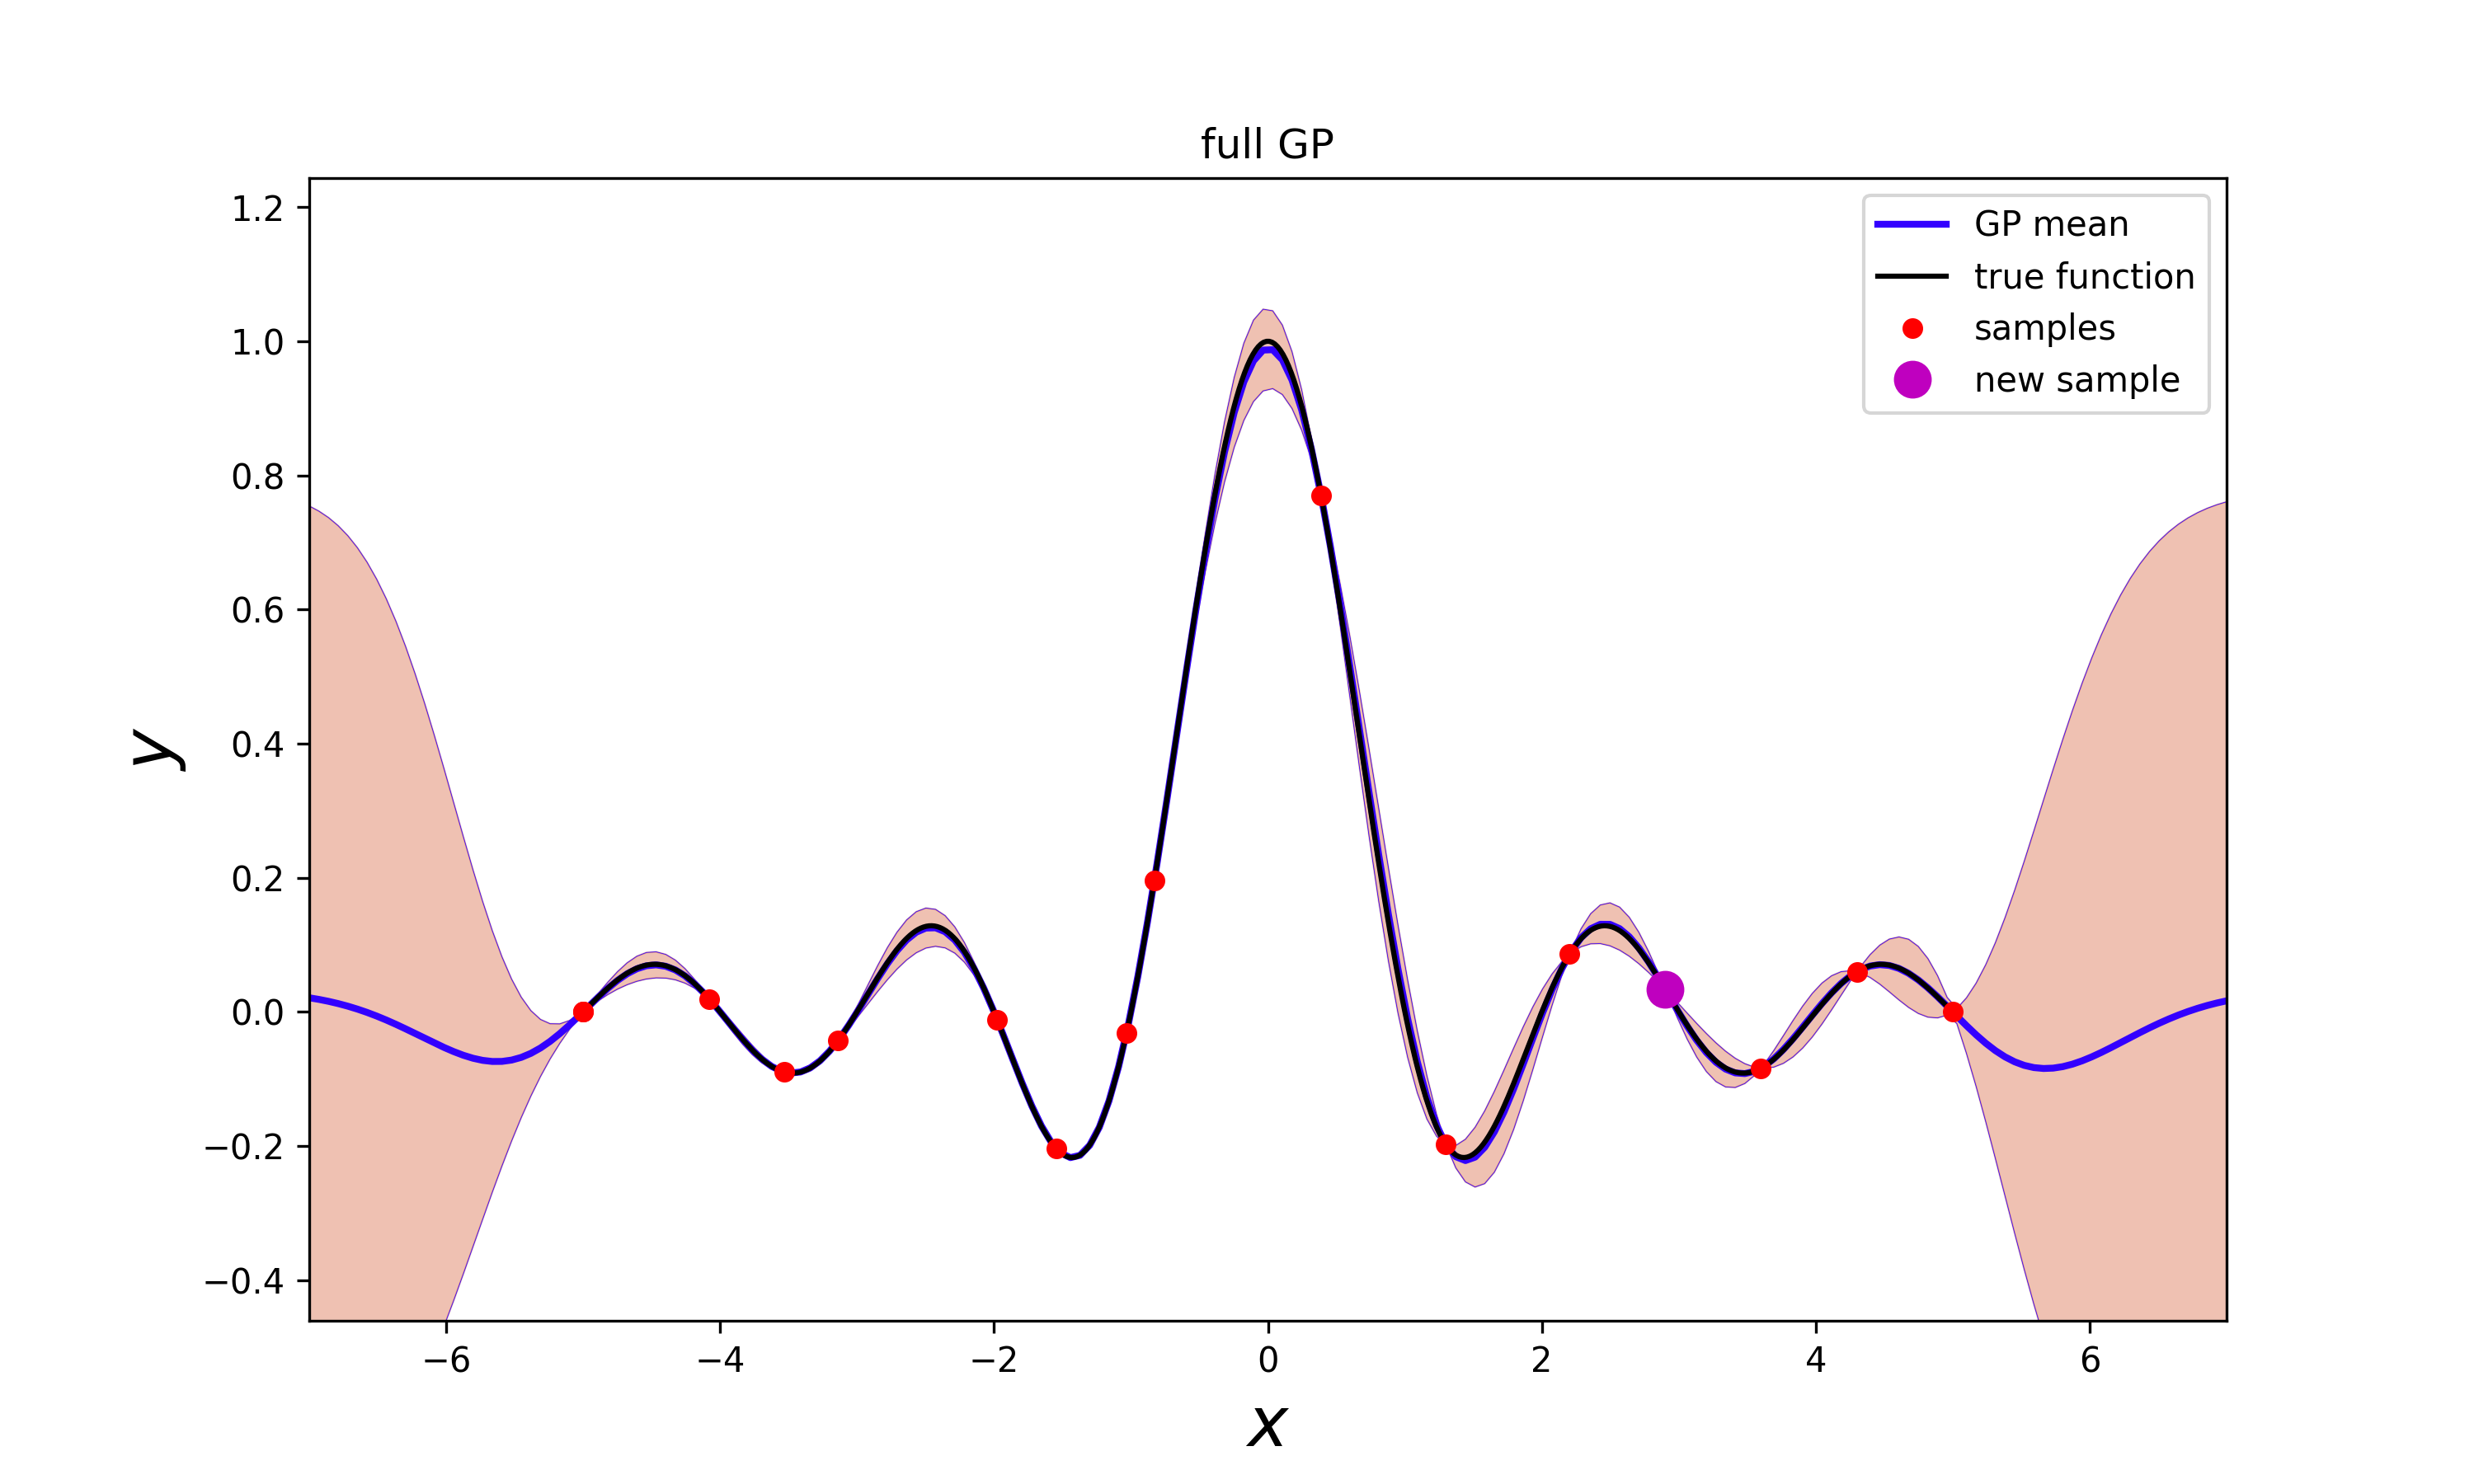
\includegraphics[width=0.74\linewidth]{final-project/update/plots/gp-12to20-pt16.png} \vspace*{-1em}
    \caption{Five iterations of variance-based active learning for a Gaussian process on the one-dimensional cardinal sine ($\text{sinc}(x)$) function on $x\in [-5,5]$ initialized with 12 random samples.}
    \label{fig:sinc-gp}
\end{figure}


\begin{figure*}[h]
    \centering
    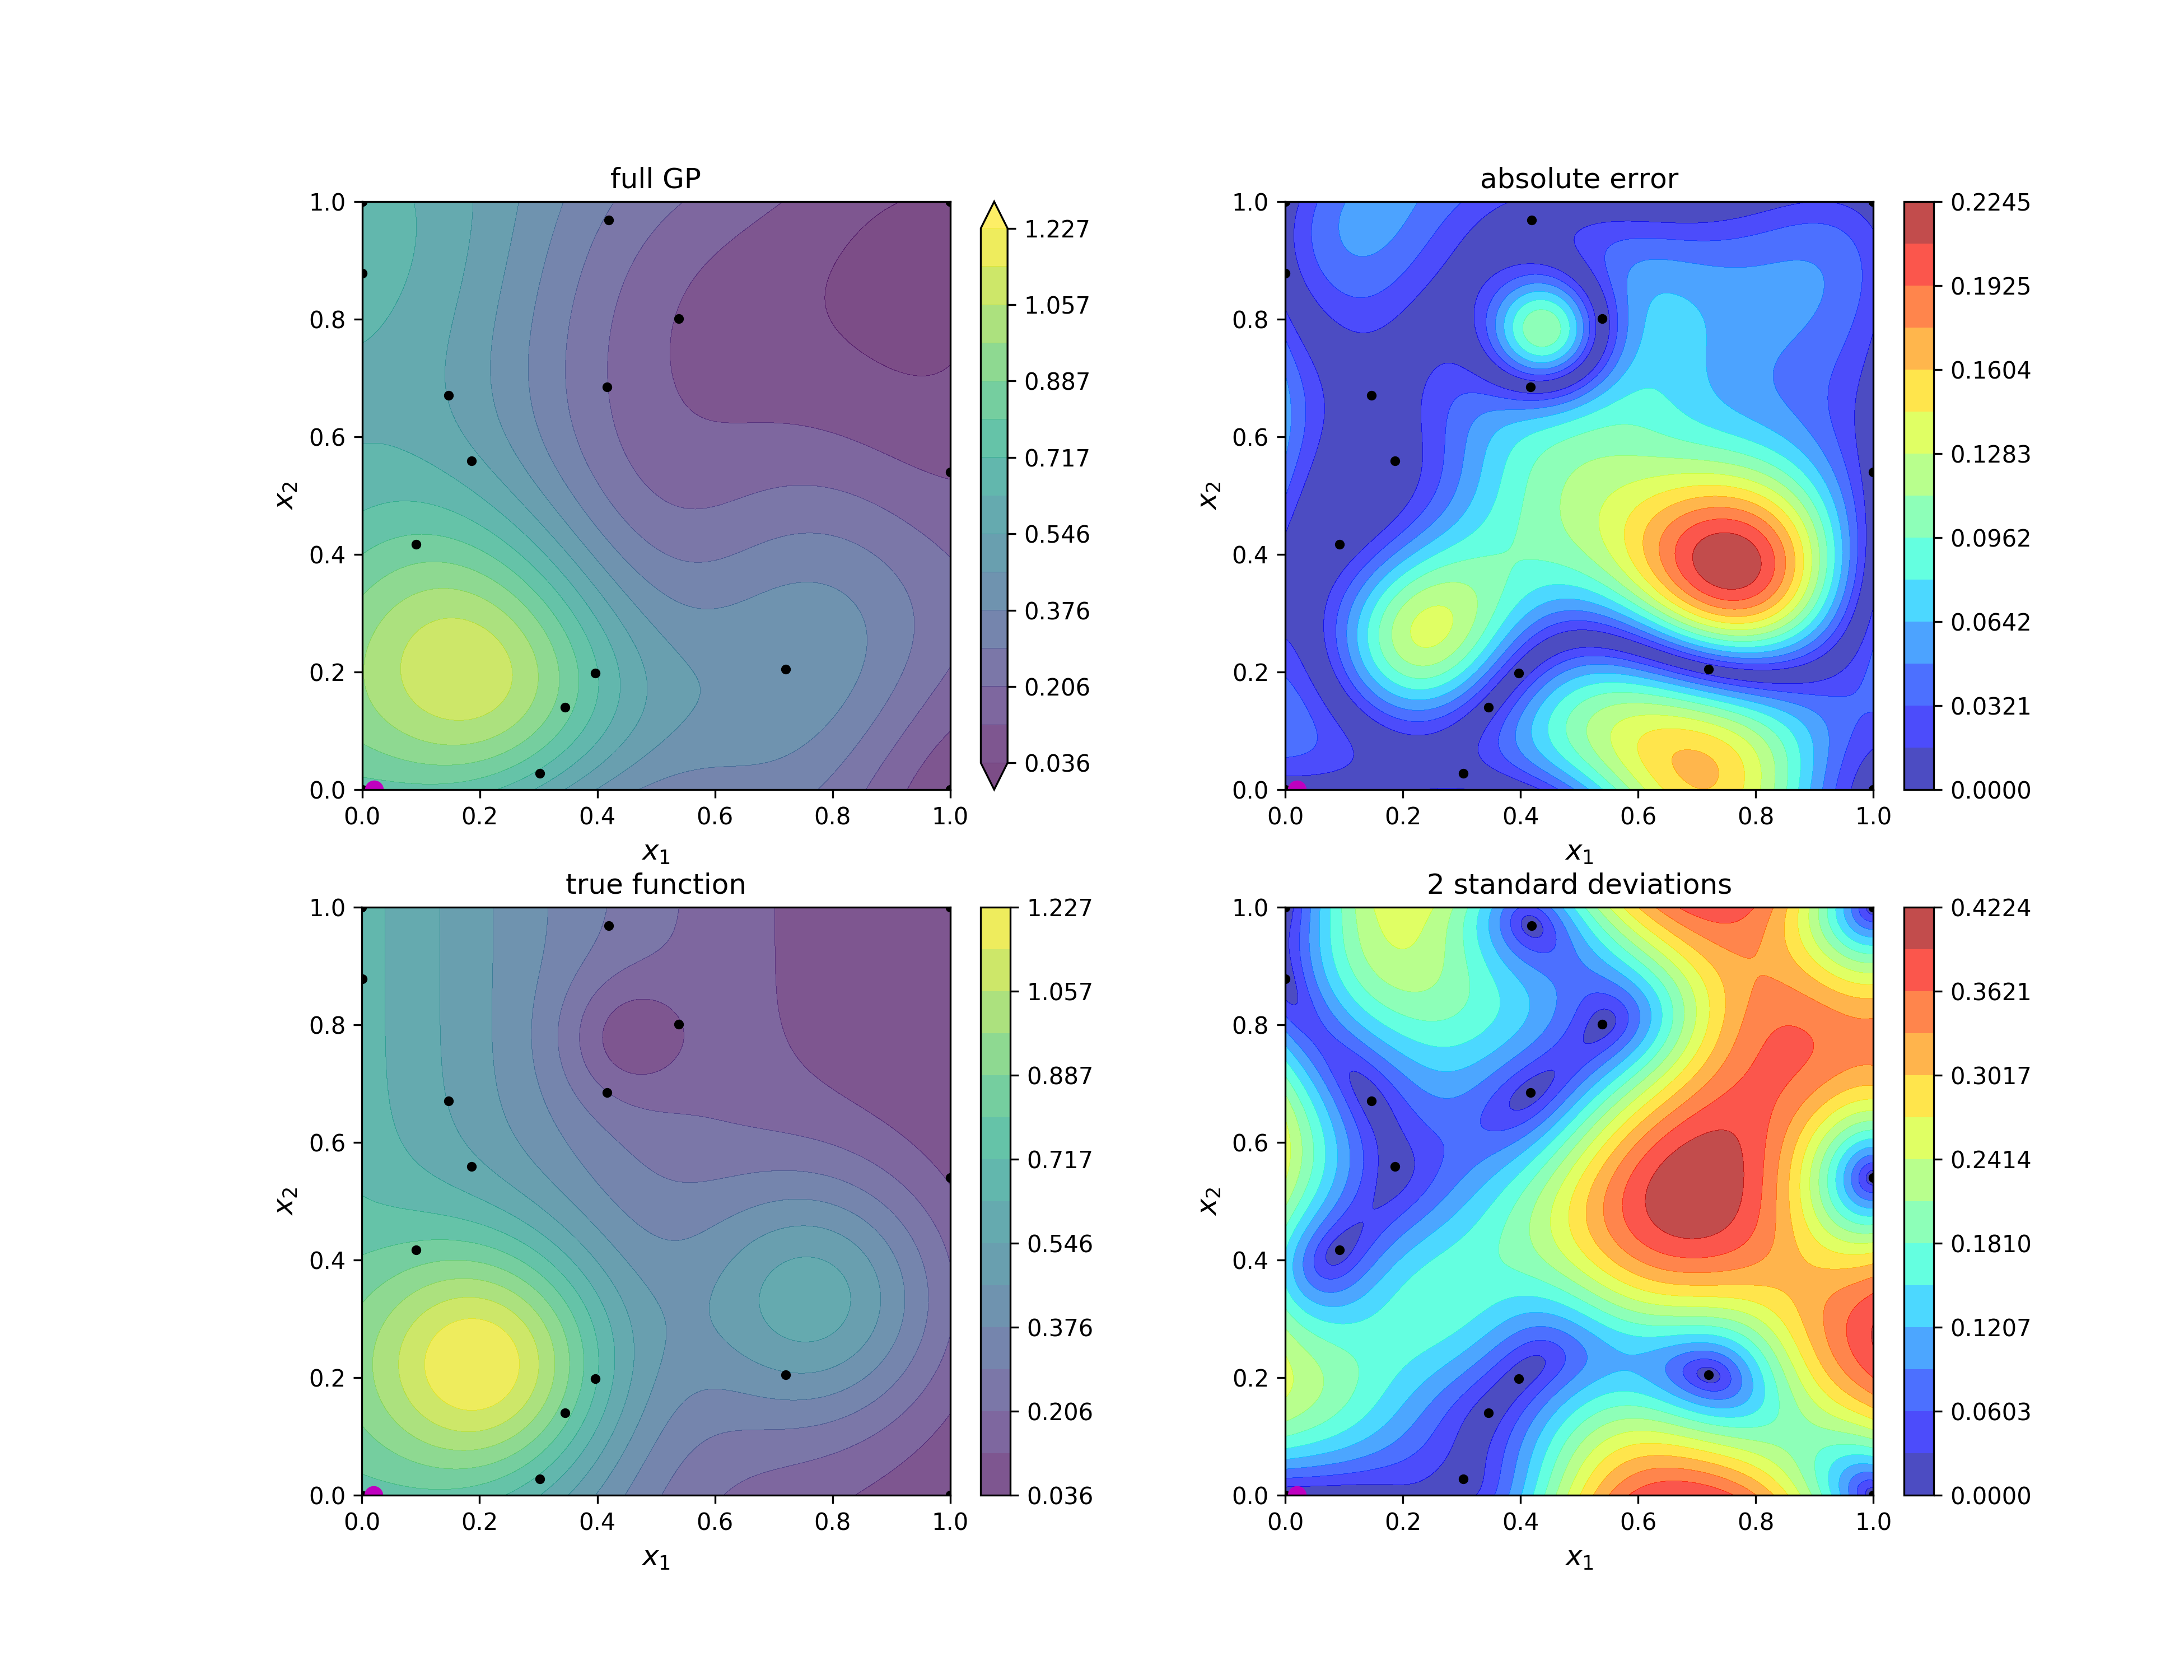
\includegraphics[width=0.99\linewidth]{final-project/update/plots/gp-20to40-pt23.png}
    \caption{A single iteration of variance-based active learning for a Gaussian process on the two-dimensional Franke function. The left plots show the predicted mean function and the true function. The right plots show the absolute error between the predicted mean function and the true function and magnitude of the two-sigma estimator from the GP.}
    \label{fig:franke-gp}
\end{figure*}


\end{document}